\documentclass[dvisvgm,tikz]{standalone}
\usepackage{circuitikz}
\begin{document}
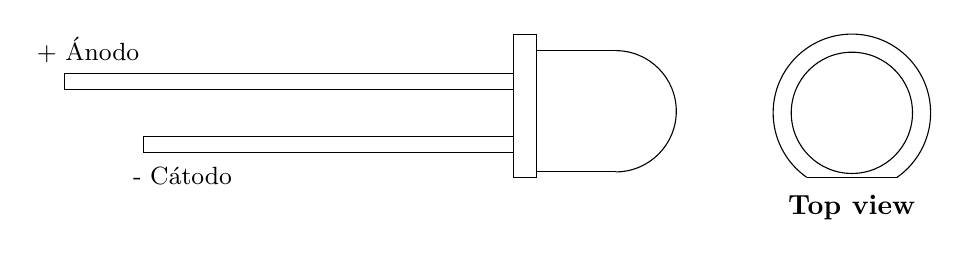
\begin{tikzpicture}
  \begin{scope}[shift={(08.0,0.75)}, rotate=180]
  \draw (0,0) arc[start angle=90, end angle=270, radius=0.77];
  \end{scope}
  \draw (07.00,2.29) -- (08.00,2.29);
  \draw (07.00,0.75) -- (08.00,0.75);
  \draw (06.70,2.50) -- (07.00,2.50);
  \draw (06.70,0.68) -- (07.00,0.68);
  \draw (07.00,0.68) -- (07.00,2.50);
  \draw (06.70,0.68) -- (06.70,2.50);
  
  \draw (2.00,1.20) rectangle (6.70,1.00);
  \draw (1.00,2.00) rectangle (6.70,1.80);
  
  \node at (1.3,2.3) {\small + Ánodo};
  \node at (2.5,0.7) {\small- Cátodo};
  
  \draw (11.00,1.50) circle (0.77);
  \coordinate (C) at (11,1.5);
  \draw (C) ++(305:1cm) arc[start angle=305, end angle=360, radius=1];
  \draw (C) ++(0:1cm) arc[start angle=0, end angle=235, radius=1];
  \draw (10.43,0.68) -- (11.58,0.68);
  
  \node at (11,0.3) {\textbf{Top view}};
\end{tikzpicture}
\end{document}